\documentclass[lang=cn,11pt]{elegantbook}
\usepackage[utf8]{inputenc}
\usepackage[UTF8]{ctex}
\usepackage{amsmath}%
\usepackage{amssymb}%
\usepackage{graphicx}
\usepackage{pdfpages}
\usepackage{biblatex}      % 用于参考文献管理
%\addbibresource{ref.bib}  % 引入 bib 文件
\newcommand*{\avint}{\mathop{\ooalign{$\int$\cr$-$}}}


\title{Notes for Math 597: advanced Real Analysis-II}
\subtitle{Following Folland' book.\cite{folland1999real}}
\setcounter{tocdepth}{2}
\author{Qiulin}
\date{Win 2025}
\extrainfo{Instructed by Professor Mattias}
\setcounter{tocdepth}{3}
%\logo{ch2-pics.assets/image-20250220154229379}
\cover{ch2-pics.assets/image-20250220154229379}

\usepackage{array}
\newcommand{\ccr}[1]{\makecell{{\color{#1}\rule{1cm}{1cm}}}}


\begin{document}
\maketitle
\frontmatter
\tableofcontents
\mainmatter


\chapter{functions of bounded variation: $F\in BV$ [Fol 3.5]}
上一节课我们证明了 Monotone Differentiation Theorem: 它表明的是, 任何 $\mathbb{R}\to \mathbb{R}$ 的 non-decreasing function 都是 differentiable a.e. 的.\\
我们知道一个函数在一整个区间上 differentiable 其实是一个比价严格的条件, 但是 differentiable a.e. 的条件就略好达到一些.\\
Question: 如果一个函数在 $[a,b] $ 上 differentiable a.e., 那么 in a.e. sense, 可以在 $[a,b] $ 上定义它的 derivative $F'$. 那么, 是否一定有 \[
F(b)  - F(a)  = \int_a^b F'(x) \, dx
\]呢? 答案肯定是不一定的. 以下是三个反例: 1. Heaviside function; 2. Cantor function; 3.$F'(x) = 0$ a.e., but not $0$ on a null set.\\
这也很显然: 因为单点的值是无法控制的. 我们只能控制 in sense of a.e. , 因而有 outlier 的 $a,b$ 是很正常的.\\
我们之后将 revisit 这一问题, 给出这个等式成立的 condition.

接下来我们将


\section{total variation function $T_F$ of a function $F$}
\begin{definition}{total variation function}
    给定一个 function $F:\mathbb{R}\to \mathbb{C}$, 我们定义它的 total variation function $T_F$ 为:\begin{align*}
        T_F : \mathbb{R} &\to [0,\infty]\\
        x &\mapsto \sup \{     \sum_{j=1}^n | F(x_j) - F(x_{j+1})| : -\infty <  x_0 < \cdots < x_n  = x    \} 
    \end{align*}
\end{definition}
\begin{remark}
    Total variation 是一个很形象的定义. $T_F(x)$ 表示的是 $F$ 从 $-\infty$ 到当前 $x$ 的这段定义域上, 总的变化量. 它 count into 所有的变化, 包括离散的和连续的, 正方向的和负方向的.\\
    \pic[0.5]{ch3-pics.assets/Screenshot 2025-04-10 at 15.39.23.png}
\end{remark}

\begin{lemma}
 对于任意的 $F:\mathbb{R}\to \mathbb{C}$,  $T_F$ 都是 increasing 的; 并且对于任意 $a<b$, 有: \[
 T_F(b) =  T_F(a) + T_F(a;b)
 \]
 where \[
 T_F (a;b) = \sup\{\sum_{j=1}^n  | F(x_j) - F(x_{j+1})| : b =  x_0 < \cdots < x_n  = a \}
 \]
表示 $F$ 的定义域限制在 $[a,b]$ 上的 total variation. 
\end{lemma}
\begin{proof}
    显然, 由于 total variation 是 increasing 的,  \textbf{我们总是可以 greedyly 选择 partition}. 对于一个 partition, 总是可以插入一个中间点把它分成两半, 而这两半的 sub partition 的 total variation 的和 $\geq$ 原先的 partition 的 total variation.
\end{proof}

\section{space of functions of bounded variation: $BV$ 的基本性质 }

\begin{definition}{function of bounded variation}
 如果 $T_F(\infty) < \infty$, 我们称 $F:\mathbb{R}\to \mathbb{C}$ is \textbf{of bounded variation} 的, 写作 $F \in BV$.
\end{definition}

\begin{definition}{function of bounded variation on an interval}
如果 $T_F(a;b) < \infty$,  我们称 $F:\mathbb{R}\to \mathbb{C}$ is \textbf{of bounded variation} on $[a,b]$, 写成 $F \in BV([a,b])$.
\end{definition}

首先显然, $F\in BV$ 可以 reduce to real-valued 的情况来讨论.
\begin{proposition}\[
    F \in BV \iff \Re f \in BV \text{ and } \Im f \in BV
    \]
\end{proposition}


\subsection{$BV$ as a vector space }

\begin{lemma}{$BV$ 是一个 complex vector space}
    如果 $F,G \in BV$, 那么对于任意的 $a,b\in \mathbb{C}$, we have \[ T_{aF + bG}  \leq |a| T_F + |b| T_G   \]
    从而$$aF + bG \in BV$$
\end{lemma}
\begin{proof}
易得. 显然, 函数的 total variation 是线性可加的.
\end{proof}

\subsection{$F\in BV$ 的 $T_F$ 的 limit behavior}

我们知道,$F\in BV$ if $T_F(\infty) < \infty$. 而关于 $ T_F(-\infty)$, 同样有强结论:
\begin{proposition} \[
F \in BV \implies T_F(-\infty)  = 0
\]
\end{proposition}
\begin{proof}
    Let $\epsilon  > 0$.\\
    从而对于任意的 $x \in \mathbb{R}$, since $F\in BV$ 那么 $T_F$ bounded, $T_F(x)$ 是一个 real number.\\
    因而我们可以找到一组 partition points $x_0 < \cdots < x_n$ 使得 \[
    \sum_{1}^n |F(x_j)- F(x_{j-1})| \geq T_F(x) - \epsilon
    \]从而 \[
    T_F(x) - T_F(x_0) \geq T_F(x) - \epsilon
    \]从而 \[
    T_F(y) \leq \epsilon,\quad \forall y\leq x_0
    \]
Since $\epsilon  > 0$ arbitrary, 这证明了 $T_F(-\infty) = 0$
\end{proof}
\begin{remark}
$F$ bounded variation 的必要条件是它在 $x \to \infty$ 时, 截止 $x$ 处的 variation $\to 0$. 
\end{remark}


\begin{lemma}{$F\in BV$ right ctn $\implies T_F$ right ctn}
$F\in BV$ right ctn $\implies T_F$ 也 right ctn
\end{lemma}
\begin{proof}
Let $x\in \mathbb{R}, \epsilon > 0$.\\
Let \[
\alpha : = T_F(x+) - T_F(x)
\]WTS: $\alpha = 0$.\\
By right ctnity of $F$ 和 $T_F$ increasing, 我们可以选择 $\delta > 0$, 同时满足: $|F(x+ h) - F(x)|<\epsilon$, $T_F(x+h) - T_F(x+) < \epsilon$ whenever $0<h<\delta$.\\
Fix 一个满足 $0<h<\delta$ 的 $h$. 其后的证明见 Folland 104.
\end{proof}




\subsection{属于 $BV,BV(I)$ 的函数 }

\begin{lemma}{哪些函数一定 $BV$ or $BV(I)$}
\begin{enumerate}
    \item 如果 $F:\mathbb{R}\to \mathbb{R}$  bounded 且 increasing, 那么  $F \in BV$ 且 $T_F(x) = F(x) - F(-\infty)$.\\
    \item 如果 $F: \mathbb{R} \to \mathbb{R}$  是 Lipschitz countinuous 的, 那么$F \in BV(I)$ for 任意的 cpt interval $I$
    \item 如果 $F: \mathbb{R} \to \mathbb{R}$  是 differentiable 且 $F'$ bounded 的, 那么 $F \in BV(I)$ for 任意的 cpt interval $I$
\end{enumerate}
\end{lemma}
\begin{proof}
(1) trivial.\\
(2) by def: 考虑 Lipschitz const $M$, 则 $T_F(a;b) \leq M (b-a)$.\\
(3): 这是 (2) 的推论, 因为 recall: by MCT 可得: $F: \mathbb{R} \to \mathbb{R}$  是 differentiable 且 $F'$ bounded $\implies F$ Lipstchiz ctn.
\end{proof}

\begin{proposition}
以下是一些经典的函数的 variational behavior: 
\begin{enumerate}
    \item $f(x) = \sin(x)$: 属于 $BV(I)$ for 任意 cpt $I$, 但不属于 $BV$.
    \item $f(x) = x\sin \frac{1}{x}, f(0) = 0$:  \textbf{属于$BV(I)$ iff $0\not\in I$.}
    \item $f(x) = x^2\sin \frac{1}{x^2}, f(0) = 0$:   \textbf{属于$BV(I)$ iff $0\not\in I$.}
\end{enumerate}
\end{proposition}
\begin{proof}
  (1) 显然;
  (2),(3) 见 HW 11. 其实它们基本相同. 
 ($\implies$): if $0 \not\in I$ then $F \in BV(I)$. 是简单的, we differentiate $F(x)=x \sin (1 / x)$ for $x \neq 0$:
$$
F^{\prime}(x)=\frac{d}{d x}\left(x \cdot \sin \left(\frac{1}{x}\right)\right)=\sin \left(\frac{1}{x}\right)+x \cdot \cos \left(\frac{1}{x}\right) \cdot\left(-\frac{1}{x^2}\right)=\sin \left(\frac{1}{x}\right)-\frac{1}{x} \cos \left(\frac{1}{x}\right)
$$
在不含 $0$ 的区间上, 它是 bounded 的. 于是 by lemma 得证.\\
($\impliedby$): if $F \in BV(I)$ then  $0 \not\in I$. This is equiv to: if $0 \in I $ then $F \not \in BV(I)$.\\
Suppose $0 \in I= [a,b] $ then $a \leq  0$ and $b \geq  0 $, one of which is strict. WLOG we suppose $b > 0$. \\
我们的 idea 是 harmonic series. 考虑
$$
y_n:=\frac{1}{n \pi+\pi / 2} \rightarrow 0^{+}
$$
we have:
$$
F\left(y_n\right)=y_n \sin \left(\frac{1}{y_n}\right)=\frac{1}{n \pi+\pi / 2} \cdot \sin (n \pi+\pi / 2)
$$For odd $n$, $F(y_n) = \frac{-1}{n \pi+\pi / 2}$, for even $n$, $F({y_n}) =  \frac{1}{n \pi+\pi / 2}$. Since $b > 0$, for some $N_0$ we have $y_{N_0} < b$. Then we consider the partition: pick $N \in \mathbb{N}$, and use $ x_0 = 0,x_1 = y_{N_0 + N-1},x_2 =y_{N_0 +N-2},\cdots, x_{N} = y_{N_0},x_{N+1} = b$ as the partition points of $[0,b]$.\\
Then we have \[
\sum_{n=1}^{N+1} |F (x_n) - F(x_{n-1}) | \geq  \sum_{n=N_0}^{N_0 -2+ N}  \frac{1}{\pi n+\pi / 2} + \frac{1}{\pi (n+1)+\pi / 2} \geq 2\sum_{n=N_0}^{N_0 -2+ N} \frac{1}{\pi n+\pi / 2}
\]
As $N \to \infty$, this sum $\sum_{n=1}^{N+2} |F (x_j) - F(x_{j-1}) |  \to \infty$, by the harmonic series.
\end{proof}



\section{Jordan decomposition for $f\in BV$: $f = \frac{1}{2}(T_F+F) - \frac{1}{2}(T_F-F)$}

\begin{lemma}
   如果 real-valued  $F \in BV$, 那么 $T_F + F, T_F - F$ 都是 increasing 的.
\end{lemma}
\begin{remark}
    $T_F + F$ 即: $F$ increasing 的地方加倍 increasing, $F$ decreasing 的地方 const;\\
     $T_F - F$ 即: $F$ decreasing 的地方反向加倍 increasing, $F$ increasing 的地方 const;
     \pic[0.5]{ch3-pics.assets/Screenshot 2025-04-10 at 15.39.58.png}
\end{remark}
\begin{proof}
    任取 $x<y$.\\
    Let $\epsilon > 0$.\\
    Can find $x_0 <  x_ 1 < \cdots < x_N = x$, s.t. \[
    \sum_{1}^N |F(x_j) - F(x_{j-1}) | \geq T_F(x) - \epsilon
    \] 从而 
    \begin{align*}
T_F(y)  &\geq    \sum_{1}^N |F(x_j) - F(x_{j-1}) |  + |F(y) - F(x)| \\
&\geq T_F(x) - \epsilon + |F(y) - F(x)|
    \end{align*}
由于 $\epsilon > 0$ 任意, 可以得到: \[
 T_F(y) -  T_F(x)\geq  |F(y) - F(x)|
\]
因而: \[
( T_F(y)  - F(y)) -  (T_F(x)  -F(x)) \geq  |F(y) - F(x)| - (F(y) - F(x)) \geq 0
\]
\end{proof} 



\begin{theorem}{Jordan decomposition for $ F \in BV $}
  对于 $F: \mathbb{R}\to \mathbb{R}$ (注意是 real-valued): \[
  F \in BV \iff F \text{ 等于两个 bounded increasing functions 的差}
  \]  Specially, \[
    F \in BV \iff  T_F \pm F \text{ bounded}
  \]
  因而 for $F\in BV$, 我们总是可以把它写作 \[
  F = \frac{1}{2}(T_F+F) - \frac{1}{2}(T_F-F)
  \]
  where we call it as the\textbf{ Jordan decomposition} of $F\in BV$. 其中,  $ \frac{1}{2}(T_F+F)$ 被称为 $F$ 的 \textbf{positive variation}; $ \frac{1}{2}(T_F-F)$ 被称为 $F$ 的 \textbf{negative variation}.
\end{theorem}
\begin{proof}
    显然, $F\in BV \implies F$ bdd, 因为\[
    |F(y) - F(x) | \leq T_F(\infty) - T_F(-\infty)
    \]
    For $F\in BV$, we have $T_F(\infty) < \infty , \; T_F(-\infty)  = 0$.\\
    又 $F\in BV \implies T_F$ bdd by def, 我们得到: \[
        F \in BV \implies  T_F \pm F \text{ bounded}
    \]而反向 trivial (bounded function 的差仍然 bounded).
\end{proof}
\begin{remark}
我们可以通过 $F$ 和 $0$ 的 min, max 取到它的正负部分, 把它按正负部分分解成 \[
F = F^+ - F^-
\]
而这里, Jordan decomposition 则是按照它正负方向上的 variation 来分: \[
  F = \frac{1}{2}(T_F+F) - \frac{1}{2}(T_F-F)
\]
$F$ 的 \textbf{positive variation}, \textbf{negative variation} 和 total variation 一样也是很形象.
\begin{figure}
    \centering
    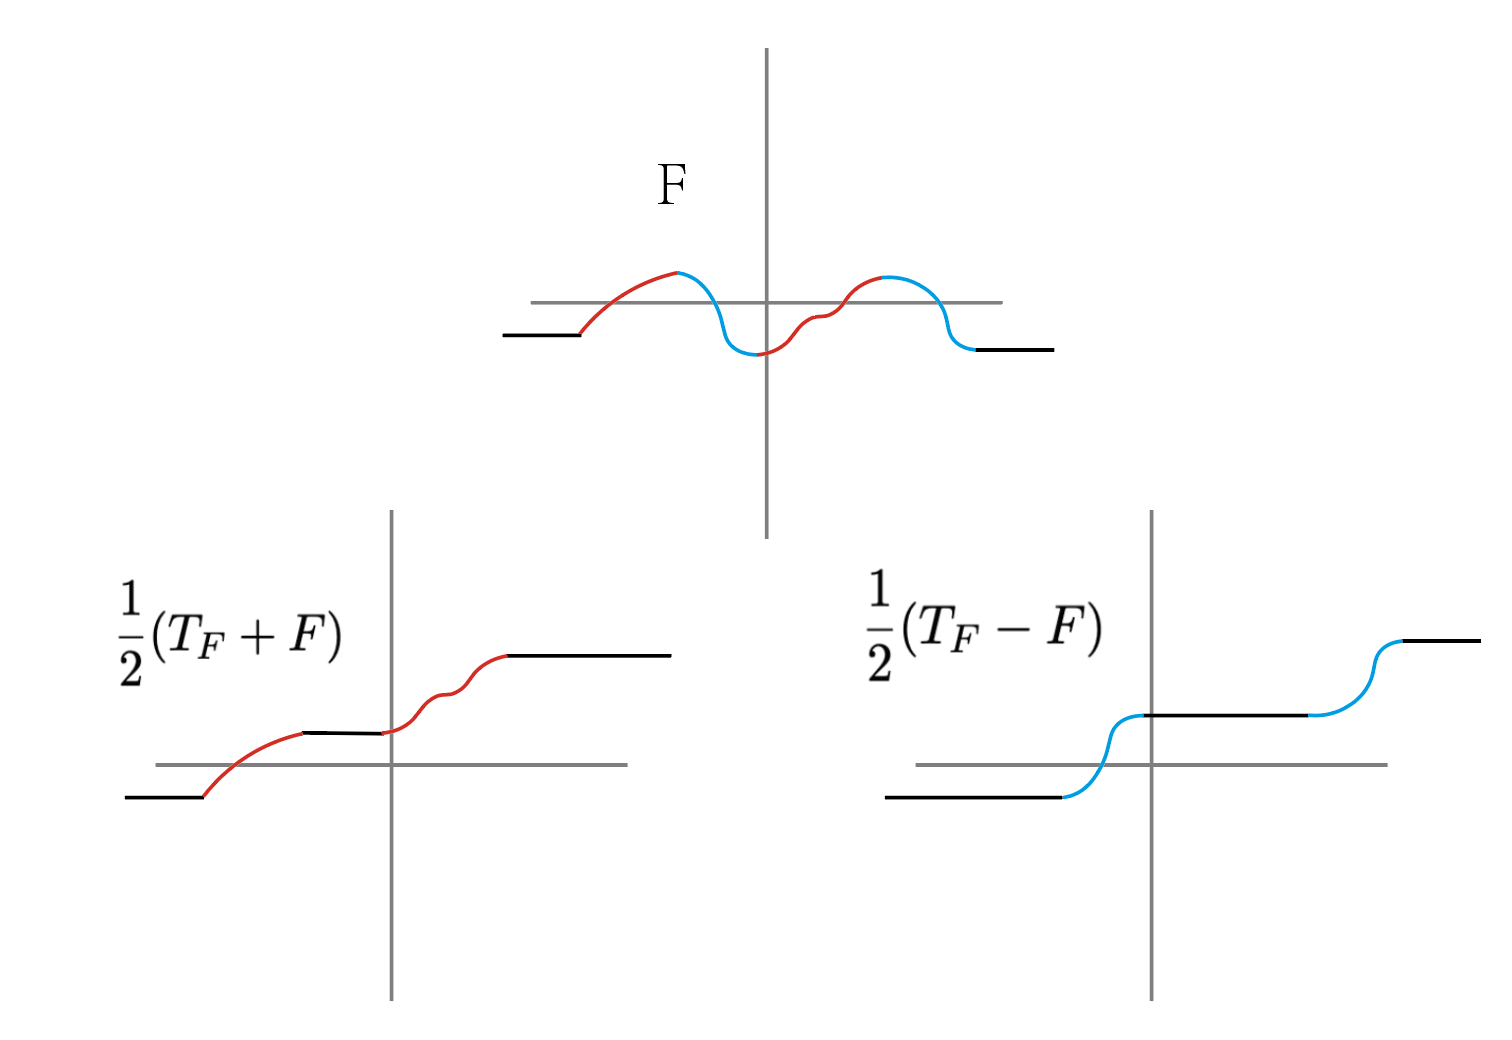
\includegraphics[width=0.5\linewidth]{lec-notes/ch3-pics.assets/Screenshot 2025-04-19 at 02.30.17.png}
    \caption{positive/negative variation} 
    \label{fig:positive/negative variation}
\end{figure}
我们把 \[
F_+ : = \frac{1}{2}T_F + F,\quad F_- : = \frac{1}{2} T_F - F
\]
(这和正负部分的拆分的记号差别在正负号的上下.)
\end{remark}

\subsection{corollaries of Jordan decomposition}
\begin{corollary}
Let $F \in BV$. By Jordan decomposition,  $F$ 等于两个 bounded increasing functions 的差.从而我们\textbf{ by MDT 得}: 
    \begin{itemize}
        \item $F(x+), F(x-)$ 存在 for all $x$; $F(\pm\infty)$ 也存在.
        \item $D_F = \{x: F \text{ disctn at }x \}$ 是 at most ctbl 的.
        \item 定义 $G (x) : = F(x+)$, 则 $F,G$ 都 a.e. differentiable 且 $F' = G'$ $m$-a.e.
    \end{itemize}
\end{corollary}
这里最重要的是: \[
F \in BV \implies F \text{ a.e. differentiable}
\]





\chapter{ $ NBV \;\&\; AC $ 空间, 以及其上的 FTC for Lebesgue integral [Fol 3.5, finished] }
\section{$NBV$ 及其性质}
\begin{definition}{NBV}
    For $F:\mathbb{R}\to \mathbb{C}$, 我们定义: $F \in NBV$, if $F \in BV$ 且 $F$ right ctn, $F(-\infty) = 0$.
\end{definition}
\begin{remark}
这个要求中 $F(-\infty) = 0$ 这一条并不要紧, 因为我们知道 for $F\in BV$, $F(-\infty) = c$ for some const $c$ 是一定的 (因为 $T_F(-\infty) =0$), 因而 right ctn 的 $F\in BV$ 减去一个常数一定是 $NBV$ 的.
    $F \in NBV$ 的
\end{remark}

\begin{proposition}
    $NBV \subset BV$ 是一个 linear subspace.
\end{proposition}
\begin{remark}
我们容易发现\[
    F \in BV \iff T_F \in BV \iff F_+, F_-  \in BV
    \]
又因为, $T_F (-\infty) = 0$ 对于 $F\in BV$ 总是成立, 且我们知道 $F$ right ctn $\implies T_F $ right ctn; 于是: \[
    F \in BV \text{ and right ctn} \implies T_F \in NBV \implies  F_+, F_- \in NBV
    \]
\end{remark}



我们已经知道:
$$\{\text{positive regular Borel measures on }\mathbb{R}\} \simeq \{\text{distribution functions }F:\mathbb{R}\to\mathbb{R} \}$$
Notice: 这一点 is achieved by 
$$
F_\mu(x ) := \begin{cases}
    \mu((0,x]) \quad  , x \geq 0 \\
     -\mu((x,0]) \; , x < 0
\end{cases}
$$
等同于: $$\mu_F ((a,b]) = F(b) - F(a)$$注意: positive regular Borel measure 和 distribution functions 都有一个共同点: 它们在 bounded set 上是 bounded 的, 但是整体可以 unbounded.\\

而现在我们证明:
\subsection{$\{\text{complex Borel measures on }\mathbb{R}\} \simeq NBV$}
注意: 一个 complex Borel measure 和一个 $F \in NBV$ 都是 finite 的.

\begin{theorem}{$\{\text{complex Borel measures on }\mathbb{R}\} \simeq NBV$}
\begin{enumerate}
    \item 对于 $\mathbb{R}$ 上的 complex measure $\mu$,  defining \[F(x) : = \mu((-\infty,x])\] 则有: \[F \in NBV\]
    \item 对于 $F \in NBV$, 一定存在某个 unique complex measure $\mu_F$ on $\mathbb{R}$, 使得 \[ \mu((-\infty,x]) = F(x) \quad \forall x \]
\end{enumerate}
\end{theorem}
\begin{proof}
    (1): 当 $\mu$ 是 positive 的情况下, 是显然的. complex 的情况就是 re/im 部分分别叠加即可.\\
    (2): 同样, WLOG 我们可以假设 $F$ 是 real-valued 的.\\
    $F\in NBV\implies F = F_+ - F_-$, 这两个都是 bounded increasing functions 且 NBV, 从而存在两个 finite signed measure 满足: \[  \mu_{\pm}((-\infty,x])  = F_{\pm}(x) - F_{\pm}(-\infty)  \] 再定义 \[\mu : = \mu_+ - \mu_-\] 即可
\end{proof}
\begin{remark}
    这里其实和 positive regular measure 关联 distribution function 的 way:
$$
F_\mu(x ) := \begin{cases}
    \mu((0,x]) \quad  , x \geq 0 \\
     -\mu((x,0]) \; , x < 0
\end{cases}
$$
是等价的, 只不过\textbf{差了一个常数 $\mu((-\infty,0])$} 而已. \\
之所以我们这里可以直接定义 \[F(x) : = \mu((-\infty,x])\]是因为, \textbf{对于 complex measure (thus finite) 而言, 这个常数 $\mu((-\infty,0])$ 一定是 finite 的. 但是对于 regular positive regular measure 而言, 这个常数可能是无穷} (且很可能). 因而对于 regular positive regular measure 我们采用这种迂回的定义方式来避开无穷值, 但是对于 complex measure 我们可以直接爽快地定义\[F(x) : = \mu((-\infty,x])\]
\end{remark}


\begin{theorem}{$\mu_F$ 的 total variation measure $=$ $\mu_{T_F}$}
    对于任意的 $F \in NBV$, 我们有: \[|\mu_F| = \mu_{T_F} \] Specially when $F$ 是 real-valued 情况下, 那么 $\mu_F$ 是一个 finite positive measure, 且有 \[\mu_{\pm} = \mu_{F_{\pm}}\]
\end{theorem}



Now: Given $F\in NBV$ with associated c.m. $\mu_F$, 什么时候 $\mu_F \perp m$, 什么时候 $\mu_F \ll m$?

\begin{theorem}{characterization of $\mu_F \perp m$ 和 $\mu_F \ll m$, for $F\in NBV$ }
    对于 $F \in NBV$, 我们已经知道: $F'$ $m$-a.e. 存在, 且 $F'\in L^1(m)$.\\
    Now we claim, 有: \[
    \mu_F \perp m \iff F' = 0 \quad m\text{-a.e.}
    \]以及 \[
        \mu_F \ll m \iff F(x) = \int_{-\infty}^x F'(t)\,d t \quad \forall x
    \]
\end{theorem}
\begin{proof}
Let $x\in \mathbb{R}$.  Applying LDT and LRNT, with $E_r: = (x,x+r]$: \[
    \lim_{r\to 0} \frac{\mu_F(E_r)}{m(E_r)} = \lim_{r\to 0} \frac{F(x+r)- F(x)}{r} = F'
    \]
    因而 $F'$ 就是这个 RN derivative. 对于 \[
    \mu_F = \lambda + \rho
    \]
    where $\lambda \perp m, \rho \ll m$, 我们有: \[F(x) : = \mu_F((-\infty,x]) =\lambda ((-\infty,x]) +\rho ((-\infty,x]) \]
我们知道, $    \mu_F \perp m \iff \rho = 0$, 从而 by LDT meets LRNT, we know that \[
F' = 0 \,\, a.e.
\]
而   $    \mu_F \ll m \iff \lambda = 0$, 从而直接 : \[F(x) : = \rho ((-\infty,x]) = F'dm((-\infty,x]) =   \int_{-\infty}^x F'(t)\,d t \]
\end{proof}



\section{$AC$ 及其性质}
\begin{definition}{absolutely continuous function}
我们定义 $F: \mathbb{R}\to \mathbb{C}$ 是 absolutely ctn 的, if 对于任意 $\epsilon > 0$ 都存在 $\delta > 0$ 使得对于任意的 disjoint intervals $(a_1,b_1),\cdots, (a_N,b_N)$, 都有: \[
\sum_1^N |F(b_j) - F(a_j)| <\epsilon \quad  \text{whenever}\quad \sum_1^N |b_j - a_j| <\delta
\]
\end{definition}
\begin{remark}
    absolutely continuous 是比 uniformly continuous 严格更强的条件: 我们只考虑 $N=1$ 而非任意正整数时这个 def 就 reduce 为 uniform ctn.\\
     absolutely continuous  表示了一种更强的控制性: 选取任意一些地方的变化足够小的 $x$, 其引发的 $y$ 的变化一定可控. ($y$ 的变化的可控性完全由 $x$ 的变化量决定, 不由 $x$ 的位置决定)\\
     这一看就和 measure 有关系.
\end{remark}
\begin{definition}{absolutely continuous function on a cpt interval}
我们定义 $F:I \to \mathbb{C}$ 是 absolutely ctn 的, if 对于任意 $\epsilon > 0$ 都存在 $\delta > 0$ 使得对于任意的 disjoint intervals $(a_1,b_1),\cdots, (a_N,b_N) \subset I$, 都有: \[
\sum_1^N |F(b_j) - F(a_j)| <\epsilon \quad  \text{whenever}\quad \sum_1^N |b_j - a_j| <\delta
\]
\end{definition}

\begin{lemma}{$F\in NBV$ abs ctn $\iff$ $\mu_F \ll m$}
    对于 $F\in NBV$, $$F \in AC\iff \mu_F \ll m$$
\end{lemma}
\begin{proof}
    我们 recall, abs ctn 除了 "$m$ 的 nullsets 也一定是 $\mu_F$ 的 null sets" 之外, 还有另一个 characterization: $\mu_F \ll m$ 当且仅当对于任意 $\epsilon > 0$ 都存在 $\delta > 0$ 使得 $ m(E) < \delta \implies|\mu_F(E)| < \epsilon$.\\
    显然, 这个 characterization 和这里的命题有关. 我们发现, $\mu_F  \ll m \implies F \in AC$ 直接 naturally follows from 这个 form. Let $\epsilon  >0$, 存在 $\delta$ 使得 $ m(E) < \delta \implies|\mu_F(E)| < \epsilon$. 那么考虑 $E = \bigsqcup_1^N (a_j,b_j)$ with $m(E) < \delta $, 直接有\[
    |\mu_F(E)|  = \sum_1^N |F(b_j) - F(a_j)| < \epsilon
    \]
从而得证.\\
而反向, 我们考虑 $m(E) = 0$, 并利用 outer regularity 取一个逼近它的 open set (每个是 union of finite disjoint open intervals) seq, 逼近 $E$, with $m(U_1) < \delta$. 由 $F \in AC$ 可以得到 \[
\mu_F(U_j) \leq \mu_F(U_1) < \epsilon
\] for all $j$, 从而 $\mu_F(E) \le \epsilon$. 从而得证, since $\epsilon $ arbitrary.
\end{proof}


\subsection{FTC-I for Lebesgue integral}
\begin{corollary}{}
    如果 $f \in L^1(m)$, 那么 \[
    F(x) : = \int_{-\infty}^x f(t) \,d t \in NBV \cap AC,\quad     f = F' \quad a.e.
    \]
Conversely, 如果 $F \in NBV \cap AC$, 那么 \[
    F' \in L^1(m), \quad F(x) = \int_{-\infty}^x F'(t) \, dt
    \]
\end{corollary}
\begin{remark}
forward 方向即: $f\in L^1(m)$ 则它的累积函数 $\int_{-\infty}^x f(t) \,d t $ 具有良好的连续性和变差有界性, 从而满足 FTC: a.e. 有 \[
\frac{d}{dx} \bigg( \int_{-\infty}^x f(t) \,d t  \bigg) = f(x)
\]
backward 方向即: 如果 $F$ 具有良好的连续性和变差有界性, 那么它的导数满足: \[F(x) = \int_{-\infty}^x F'(t) \, dt    \]
简而言之: \textbf{FTC-I for Lebesgue integral 在整个 $\mathbb{R}$ 上都成立当且仅当 $F \in NBV \cap AC$.}
\end{remark}


\subsection{FTC-II for Lebesgue integral on a cpt interval}
比起刚才的 FTC-I, FTC-II 的条件要宽松很多, 只需要 $F$ 在它需要被用到的 compact interval 上 AC 即可以. 这是因为, 我们不需要用到 NBV 只需要 BV, 并且在 cpt interval 上, AC 本身就可以推出 BV.
\begin{lemma}
    如果 $F\in AC([a,b])$, 那么 $F\in BV([a,b])$.\\
    即 \[
    AC([a,b]) \subset BV([a,b])
    \]
\end{lemma}
\begin{proof}
    这是显然的. 我们看到 $F \in AC([a,b])$ 的定义: on $[a,b]$ we have: \[
\sum_1^N |F(b_j) - F(a_j)| <\epsilon \quad  \text{whenever}\quad \sum_1^N |b_j - a_j| <\delta
\]
我们不妨考虑 $\epsilon = 1$, 然后可以划分 $[a,b]$ into 一个个总长度为 $\frac{\delta}{2}$ 的由 disjoint intervals 构成的块 (补空缺没事), 从而 Bound 住这个划分上的 variation by parition \(\sum_1^{N_0} |F(b_j) - F(a_j)| \). 而我们发现: 这个时候我们不论怎么 fine 这个划分, 每个块的总长度总归是不变的, 从而仍然可以使用原先的 bound.\\
我们 recall: for total variation, partition 的选取是 greddy 的. 从而这就足以得证.
\end{proof}
\begin{remark}
这里没有仔细证明, 但是理解这个 idea 即可. 这表现了 locally, $AC$ 是一个比 $BV$ 更强的条件, 因为 total variation 就是 sup of variations over 所有划分, 而 \textbf{$AC$ 的定义正好就是: 无视划分的方法, 只要这个集合的总长度小于 $\delta$, 它上面的 variation by partition 就要小于 $\epsilon$. }
\end{remark}

\begin{theorem}{FTC-II for Lebesgue integral on a cpt interval}
TFAE:
\begin{itemize}
    \item $F\in AC[a,b]$
    \item $F$ 是 diffble a.e. on $[a,b]$ 的, 并且 $F'\in L^1([a,b],m)$, 并且 \[F(x) - F(a) = \int_a^x F'(t)\, dt\]\textbf{for all $x\in [a,b]$}.
\end{itemize}
\end{theorem}
\begin{proof}
    首先
\end{proof}


\chapter{distribution function of a function and Chebshev's ineq on $L^p$}
我们

$$
F_\mu(x ) := \begin{cases}
    \mu((0,x]) \quad  , x \geq 0 \\
     -\mu((x,0]) \; , x < 0
\end{cases}
$$
是等价的, 只不过\textbf{差了一个常数 $\mu((-\infty,0])$} 而已. \\
之所以我们这里可以直接定义 \[F(x) : = \mu((-\infty,x])\]




\chapter{Problem solving}
Recall: Given mspace $(X,\mathcal{A},\mu)$ 以及 $f:X \to \mathbb{C}$ mble, 我们可以 define distribution function: \[
\lambda_f : (0,\infty) \to [0,\infty]
\]
by \[
\lambda_f (\alpha) = \mu(\{\mathbb{}|f| > \alpha \} )
\]
Chebyshevs ineq: \[
\lambda_f(\alpha) \leq  \bigg(\frac{\| f\|_p}{\alpha} \bigg)^p
\]for $0< p < \infty$.\\
Today: Problem Solving



\begin{proposition}
    对于任意 $0< p < \infty$, 我们有: \[
    \int_X |f|^p \, d\mu = \int_0^\infty p \alpha^{p-1} \lambda_f (\alpha ) \, d\alpha
    \]
\end{proposition}
左边是 integral on $X$, 右边是 integral on $\mathbb{R}$.

\begin{proof}
    Sketch: 
    Step 1: $f$ simple $\implies$ $|f|$ simple.\\
    
\end{proof}

Write \[
|f| = \sum_{j=1}^N c_j \chi_{A_j} 
\]where $A_j$ disjoint, $c_1 > c_2 > \cdots >  c_N > 0$
This implies: \[
\int |f| ^p \, d\mu = \sum_{j=1}^N c_j^p r_j,\quad r_j = \mu(A_j)
 \]
Then
\begin{align*}
\lambda_f (\alpha) = \begin{cases}
    \sum_{j=1}^N r_j,& 0 < \alpha < c_N\\
    \sum_{j=1}^{n-1} r_j,&c_n \leq \alpha  < c_{n-1}, 2\leq n \leq N\\
    0,& \alpha \geq c_1
\end{cases}    
\end{align*}
从而 
\begin{align*}
    \int_0^\infty p \alpha^{p-1} \lambda_f (\alpha) d\alpha & = (\sum_{j=1}^N r_j) \int_0^{c_N} p \alpha^{p-1} d\alpha + \sum_{n=2}^N (\sum_{j=1}^{n-1} r_j ) \int_{c_n}^{c_{n-1}} p\alpha^{p-1} \, d\alpha\\
    & = 
\end{align*}


Step 2: $f$ general.\\
Use: $\exists$ simple functions $g_n \geq 0$ s.t. $g_n \nearrow |f|$.\\
 MCT $\implies $ \[
 \int_X |f|^p \,d \mu = \lim_{n\to \infty} \int_X g_n^p \, d\mu
 \]
 Also, \[
\lambda_{g_n} \overset{\text{CFB} }{\nearrow  }  \lambda_f \quad \text{pointwisely on} (0,\infty)
 \]
从而  MCT $\implies $ \[
\lim_{n\to \infty} \int_0^\infty p\alpha^{p-1} \lambda_{g_n}(\alpha) \, d\alpha \to \int_0^\infty p \alpha^{p-1} \lambda_f (\alpha ) \, d\alpha
\]
$\lambda_f(\alpha) = \mu(\{ |f| > \alpha\})$, 以及 $\{ |f| > \alpha \} = \bigcup_1^\infty \{g_n > \alpha \} $ increasing union.




\begin{example}
    Let $f:[0,1] \to \mathbb{R}$ be abs ctn. Suppose $f(0)  = 0$ 以及 $f^1 \in L^2([0,1])$.\\
    Show that the limit \[
    \lim_{x \to 0^+} x^{-1/2} f(x)
    \]exists, 并 compute it.\\
    What could the limit be? Must be $0$.\\
\begin{solution}
    Use FTOC, can recover $f$ from $f'$.\\
    \[
    f(x) = f(0) + \int_0^x f'(t) \, dt,\quad 0\leq x \leq 1
    \]
    使用 Hölder with $p=q =2$ (Cauchy-Swartz): \[
    |f(x)| \leq \int_0^x |f'(t)| \, dt = \int_0^x |f'(t) | 1\, dt  \leq \bigg(\int_0^x |f'(t)|^2\bigg)^\frac{1}{2} x^{\frac{1}{2}}
    \]
    从而 \[
    x^{-1/2} |f(x)| \leq \int_0^x |f'(t) | ^2 \, dt 
    \]
    Use fact: \(    g = L^1 (X,\mathcal{A},\mu) \implies \forall \epsilon > 0, \exists \delta > 0\) s.t. for all $\mu(E) < \delta $ we have $\int_E |g| \, d\mu < \epsilon$.\\
  (Proof of this fact: use approx by simple functions 可得).\\
  然后 use approx by simple functions, apply to $g = |f'|^2$, $\mu = m$, $E = [0,x]$, 于是得到 \[
  \int_0^x |f'(t)| ^2 dt \overset{x\to 0}{\longrightarrow} 0
  \]
\end{solution}
\end{example}


\begin{example}
    Let $f: \mathbb{R}^n \to \mathbb{R}$ be a function.\\
    Assume: 对于 $\forall \epsilon > 0$, 都存在 Lebesgue mble functions $g,h\in L^1 (m)$  s.t. \[
    g(x) \leq f(x) \leq h(x) \quad \forall x \in \mathbb{R}^n
    \]并且 \[
    \int_{\mathbb{R}^n} (h-g) \, dm < \epsilon 
    \]
    Prove that: $f$ 也是 Lebesgue mble 的, 并且 $f\in L^1(m)$.\\
   \begin{proof}
By assumption: Given $k \in \mathbb{N}$, 存在 $g_k,h_k \in L^1(\mathbb{R}^n)$ s.t.  \[   g_k \leq f \leq h_k ,\quad \int (h_k - g_k) < \frac{1}{k}\]
Idea: $f = \limsup g_k = \liminf h_k$ ? \\
我们应该 try to prove: for a.e. $x$ 都有 $ 0\leq h_k(x) - g_k (x) \to 0$.\\
Use Fatou's Lemma: \[
\int \liminf_{k\to \infty} (h_k - g_k) \leq \liminf_{k\to \infty} \int (h_k - g_k)  = 0
\]而 $h_k - g_k \geq 0$, 因而 This means: \[
 \liminf_{k\to \infty} (h_k - g_k) = 0\quad \text{for a.e. } x
\]
且我们知道\[
\liminf_{k\to \infty} (h_k - f)\leq \liminf_{k\to \infty}  (h_k - g_k) = 0\quad \text{for a.e. } x
\]
从而 \[
f(x) = \liminf_{k\to \infty} h_k(x) \quad \text{for a.e. } x
\]
This proves that, $f$ is Lebesgue measurable.
   
   \end{proof}
\end{example}









\begin{example}
    Prove that: \[
    \lim_{n\to \infty} \int_E \sin (nx)\, dx = 0
    \]for every bounded Borel set $E \subset \mathbb{R}$.\\
\begin{proof}
    Step 1: $E = (a,b)$ 是一个 interval.\\
    \begin{align*}
        \int_E \sin (nx)\,d x  & = \bigg[ -\frac{1}{n} \cos (nx)   \bigg]_a^b
    \end{align*}
    从而 \[
       \bigg|   \int_E \sin (nx)\,d x  \bigg| \leq \frac{2}{n} \overset{n\to \infty}{\longrightarrow } 0
    \]
    Step 2: $E$ 是一个 finite union of disjoint open intervals.\\
    Same as Step 1.\\
    Step 3: General Case.\\
    Fix $\epsilon > 0$.\\
    Then by outer regularity: 存在 some $U$ 为 finite disjoint union of open intervals, 使得 \[
    m(U \Delta E ) < \epsilon
    \]
    从而 \[
\bigg| \int_E f_n = \int_U f_n   \bigg| < \bigg|\int_{U \Delta E} f_n\bigg| \leq m(U \Delta E) < \epsilon
    \]因而\[
 \bigg|\int_{ E} f_n\bigg|  <   \bigg|\int_{ U} f_n\bigg| + \epsilon
    \]for all $n$. 并且 By step 2: \[
    \limsup_{n\to \infty} \bigg | \int _U f_n \bigg| + \epsilon = 0 + \epsilon
    \]
    因而 \[    \limsup_{n\to \infty} \bigg | \int _E f_n \bigg| \leq \epsilon \]
    Since $\epsilon$ arbitrary, 得证.
\end{proof}
\end{example}






\begin{example}
    Let $E \subset \mathbb{R}$ be a Borel set, with $m(E) > 0$.\\
    Set $f: \mathbb{R}\to \mathbb{R}$ be mble, nonneg, 并且 $\int f > 0$.\\
    Prove that: 存在 $t \in \mathbb{R}$ s.t. $$\int_{E + t} f > 0$$
    \begin{proof}
\textbf{Claim 1: STS to assume $f$ simple.}\\
Proof of Claim 1: 对于 $f$, can find seq of simple functions $0 \leq f_n \leq f$, s.t. $f_n \nearrow f$.\\
By MCT, 
    \end{proof}
\end{example}





\chapter{problem solving-III}

\begin{example}
    Let $f \in L^2_{loc} (\mathbb{R})$.\\
    Assume \[
    \int_a^a |t||f(x+t)|\, dt \geq \frac{2}{\sqrt{3}}a^2
    \]for all $a> 0$, $x\in\mathbb{R}$.\\
Now show: $|f(x)| \geq 1$ for a.e. $x$.\\
\begin{proof}
    WLOG 可以假设 $f$ 是 nonneg 的. ($f\mapsto |f|$).\\
    WTS: $|f(x)| \geq 1$ for a.e. $x$. \\
Claim 1: by LDT, it STS: \[
\frac{1}{2a} \int_{-a}^a  f(x+t)\, dt  \geq 1
\]for all $x\in \mathbb{R}$.\\


我们 try Cauchy Swartz:
\[
\int_{-a}^a  |t| f(x+ t) \, dt \leq \bigg(\int_{-a}^a t^2 \, dt   \bigg)^{1/2} \bigg(\int_{-a}^a   f(x+t)^2 \, dt   \bigg)^{1/2}
\]
我们知道: 左边 $\geq \frac{2}{\sqrt{3}} a^2$, 而右边第一项 $(\int_{-a}^a  t^2 \, dt   )^{1/2}$ 是可以计算的: 等于 $(\frac{2a^3}{3})^{1/2}$.\\
于是, 我们得到 \[
\int_{-a}^a  f(x+t)^2 \, dt \geq 2a
\]
从而: 
\[
\frac{1}{2a}\int_{-a}^a  f(x+t)^2 \, dt \geq 1
\]
然后 by LDT: \[
\frac{1}{2a}\int_{-a}^a  f(x+t)^2 \, dt = \frac{1}{2a}\int_{x-a}^{x+a}  f(y)^2 \, dy =    f(x)
^2 \]
for a.e. $x$. 因而 \[
 f(x)^2 \geq 1\,\quad \text{for a.e. }  x
\]于是 \[
| f(x)| \geq 1\,\quad \text{for a.e. }  x
\]
\end{proof}
\end{example}





\begin{example}
    Prove or disprove: 对于 bounded open set $E \subset \mathbb{R}$, 它的 boundary 是否一定满足 $m(\partial E) = 0$ ? \\
    \begin{solution}
        Astonishingly 这个问题的回答是否定的. 我们可以构造
    \end{solution}
\end{example}



 


\chapter{extra topics}

\section{Minkowski ineq for integral}



\section{convolution}
我们已经证明了, for $1\leq p< \infty$, \[
C_c^0(\mathbb{R}^n)  \subset L^p(\mathbb{R}^n) \quad\text{dense subset}
\]What about for $p = \infty$? 答案也是 true 的, 我们需要用到 convolution 来证明.\\







\printbibliography
\appendix





\end{document}